\documentclass[10pt,a4paper]{article}

% -------------------------------------------------
% Packages
% -------------------------------------------------
\usepackage[T1]{fontenc}
\usepackage[utf8]{inputenc}
\usepackage[english]{babel}
\usepackage[a4paper,margin=2cm]{geometry}
\usepackage{microtype}
\usepackage{setspace}
\setstretch{1.04}

\usepackage{amsmath,amssymb,amsfonts,mathtools,bm}
\usepackage{amsthm}
\usepackage{graphicx}
\usepackage{subcaption}
\usepackage{booktabs}
\usepackage{multirow}
\usepackage{array}
\usepackage{tikz}
\usepackage[most]{tcolorbox}
\usepackage{enumitem}
\usepackage{hyperref}
\usepackage{titlesec}
\usepackage{caption}
\usepackage{fancyhdr}

% -------------------------------------------------
% Colors
% -------------------------------------------------
\usepackage{xcolor}
\definecolor{TitleColor}{HTML}{102A43}
\definecolor{AccentColor}{HTML}{2F80ED}
\definecolor{SoftBlue}{HTML}{EAF2FF}
\definecolor{SoftGray}{HTML}{F7F9FC}
\definecolor{TextGray}{HTML}{3A3A3A}

\hypersetup{
    colorlinks=true,
    linkcolor=AccentColor,
    citecolor=AccentColor,
    urlcolor=AccentColor
}

% -------------------------------------------------
% Section style
% -------------------------------------------------
\titleformat{\section}
    {\Large\bfseries\color{TitleColor}}
    {\thesection}{0.6em}{}
\titleformat{\subsection}
    {\large\bfseries\color{TitleColor}}
    {\thesubsection}{0.6em}{}

% -------------------------------------------------
% Caption style
% -------------------------------------------------
\captionsetup{
    font=small,
    labelfont={bf,color=TitleColor},
    labelsep=period
}

% -------------------------------------------------
% Header
% -------------------------------------------------
\pagestyle{fancy}
\fancyhf{}
\lhead{\textcolor{TextGray}{Flow Matching Project}}
\rhead{\textcolor{TextGray}{MVA 2025--2026}}
\cfoot{\thepage}
\renewcommand{\headrulewidth}{0.25pt}

% -------------------------------------------------
% Theorems
% -------------------------------------------------
\newtheorem{theorem}{Theorem}
\newtheorem{proposition}{Proposition}
\newtheorem{lemma}{Lemma}
\theoremstyle{definition}
\newtheorem{definition}{Definition}
\newtheorem{remark}{Remark}

% -------------------------------------------------
% Commands
% -------------------------------------------------
\newcommand{\R}{\mathbb{R}}
\newcommand{\E}{\mathbb{E}}
\newcommand{\cN}{\mathcal{N}}
\newcommand{\cL}{\mathcal{L}}
\newcommand{\dd}{\mathrm{d}}
\newcommand{\norm}[1]{\left\lVert #1 \right\rVert}
\newcommand{\Id}{\mathrm{Id}}

% -------------------------------------------------
% Boxes
% -------------------------------------------------
\newtcolorbox{highlightbox}{
    colback=SoftBlue,
    colframe=AccentColor,
    boxrule=0.8pt,
    arc=2mm,
    left=1.5mm,right=1.5mm,top=1.2mm,bottom=1.2mm
}

\newtcolorbox{takeawaybox}{
    colback=SoftGray,
    colframe=TitleColor,
    boxrule=0.6pt,
    arc=2mm,
    left=1.5mm,right=1.5mm,top=1.2mm,bottom=1.2mm
}

% -------------------------------------------------
% Title block
% -------------------------------------------------
\begin{document}

\begin{center}
    {\LARGE\bfseries\color{TitleColor}
    On the Closed-Form of Flow Matching}\\[0.25em]
    {\large\bfseries\color{TitleColor}
    Generalization Does Not Arise from Target Stochasticity}\\[0.9em]

    {\large Gaspard Beaudouin \hspace{1cm} Yentl Collin}\\[0.25em]
    {\normalsize Master MVA, \'Ecole Normale Sup\'erieure Paris-Saclay}\\[0.25em]
    {\normalsize Generative Modeling (2025--2026)}
\end{center}

\vspace{0.5em}

\begin{highlightbox}
\textbf{Project goals.}
We investigate the theoretical and empirical relationship between Flow Matching and diffusion models.
We reproduce key phenomena from the paper~\cite{bertrand2025closed} on synthetic datasets and study how the generalization switching time depends on dataset geometry, dimension, time schedule, and model capacity.
\end{highlightbox}

%==========================================================================
\section{Introduction}
%==========================================================================

Deep generative models have achieved remarkable success in synthesizing realistic data, from images~\cite{ho2020denoising} to audio and video.
Among recent approaches, \emph{diffusion models}~\cite{song2021score,ho2020denoising} and \emph{flow matching} (FM)~\cite{lipman2023flow,liu2023flow,albergo2023building} have emerged as the two dominant frameworks.
Both define a probability path $(p_t)_{t\in[0,1]}$ from a simple source distribution $p_0 = \cN(0,\Id)$ to a data distribution $p_1 = p_{\mathrm{data}}$, then learn dynamics whose time marginals follow this path.

A central and puzzling question is: \emph{why do these models generalize rather than memorize the training data?}
Bertrand et al.~\cite{bertrand2025closed} challenge the hypothesis that generalization stems from the noisy/stochastic nature of the conditional FM loss.
Leveraging the closed-form expression of the optimal empirical velocity field $\hat{u}^\star$, they show that (i)~in high dimensions, $\hat{u}^\star$ is effectively non-stochastic for most of the flow trajectory, and (ii)~generalization arises when the limited-capacity neural network $u_\theta$ fails to approximate $\hat{u}^\star$, particularly at early times.

\paragraph{Contributions.}
In this project, we:
\begin{enumerate}[leftmargin=1.5em,nosep]
    \item Present the theoretical equivalence between flow matching and diffusion models (Section~\ref{sec:background}--\ref{sec:equivalence}).
    \item Reproduce the three main figures of~\cite{bertrand2025closed} on toy datasets: the stochasticity analysis (Figure~1), velocity approximation failure (Figure~2), and the generalization switching time (Figure~3).
    \item Go beyond the paper by systematically varying dataset geometry, dimension, model capacity, and training duration to characterize how each factor influences the switching time.
\end{enumerate}

All experiments run on a single Google Colab T4 GPU in under 30 minutes per notebook.

%==========================================================================
\section{Background}\label{sec:background}
%==========================================================================

\subsection{Diffusion models}

Diffusion models define a \emph{forward process} that gradually adds noise to data via a stochastic differential equation (SDE):
\begin{equation}\label{eq:forward-sde}
    \dd X_t = f(X_t, t)\,\dd t + g(t)\,\dd W_t, \qquad X_0 \sim p_{\mathrm{data}},
\end{equation}
where $f$ is a drift, $g(t)$ is a scalar diffusion coefficient, and $W_t$ is a standard Brownian motion.
For a linear SDE with $f(x,t) = f_t\, x$, the conditional law of $X_t$ given $X_0 = x_0$ is Gaussian:
\[
    X_t \mid X_0 = x_0 \;\sim\; \cN(\alpha_t\, x_0,\; \sigma_t^2\, \Id),
\]
where $\alpha_t = \exp(\int_0^t f_s\,\dd s)$ and $\sigma_t^2 = \alpha_t^2 \int_0^t g_s^2\, \alpha_s^{-2}\,\dd s$.
The marginal density $p_t$ of $X_t$ evolves according to the Fokker--Planck equation:
\begin{equation}\label{eq:fp}
    \partial_t p_t = -\nabla\cdot(p_t\, f) + \frac{g(t)^2}{2}\,\Delta p_t.
\end{equation}

\paragraph{Reverse-time SDE.}
To generate new data, one reverses the forward process.
The reverse-time SDE reads:
\begin{equation}\label{eq:reverse-sde}
    \dd \bar{X}_\tau = \Big[-f(\bar{X}_\tau, T-\tau) + g(T-\tau)^2\,\nabla\log p_{T-\tau}(\bar{X}_\tau)\Big]\dd\tau + g(T-\tau)\,\dd\bar{W}_\tau,
\end{equation}
which requires the \emph{score function} $\nabla_x \log p_t(x)$.
Since the marginal score is intractable, one uses the identity
\begin{equation}\label{eq:score-cond}
    \nabla_x \log p_t(x) = \E\!\big[\nabla_x \log p_t(x \mid X_0) \;\big|\; X_t = x\big],
\end{equation}
which reduces score estimation to a regression problem.
The \emph{denoising score matching} loss trains a network $s_\theta$ with:
\[
    \cL_{\mathrm{DSM}}(\theta) = \E_{t,\,x_0,\,\varepsilon}\!\Big[\norm{s_\theta(\alpha_t x_0 + \sigma_t \varepsilon,\, t) + \frac{\varepsilon}{\sigma_t}}^2\Big].
\]

\paragraph{Probability-flow ODE.}
Crucially, there exists a \emph{deterministic} ODE sharing the same marginals~$p_t$ as the SDE:
\begin{equation}\label{eq:pf-ode}
    \frac{\dd}{\dd t}\tilde{X}_t = f(\tilde{X}_t, t) - \frac{g(t)^2}{2}\,\nabla\log p_t(\tilde{X}_t).
\end{equation}
This probability-flow ODE is the bridge to flow matching.

\subsection{Flow Matching}\label{subsec:fm}

Flow matching~\cite{lipman2023flow} directly learns a velocity field $u:\R^d\times[0,1]\to\R^d$ such that the ODE
\begin{equation}\label{eq:fm-ode}
    \dot{x}(t) = u(x(t), t), \qquad x(0) \sim p_0 = \cN(0, \Id),
\end{equation}
transports $p_0$ to $p_{\mathrm{data}}$.
By the mass conservation criterion, this holds if and only if $(p_t, u)$ satisfies the continuity equation $\partial_t p_t + \nabla\cdot(p_t\, u) = 0$.

\paragraph{Conditional paths.}
FM constructs a probability path through conditioning.
Given $z = x_1 \sim p_{\mathrm{data}}$, define the conditional path
\begin{equation}\label{eq:cond-path}
    p_t(\cdot \mid x_1) = \cN\!\big(t\, x_1,\; (1-t)^2\,\Id\big),
\end{equation}
with conditional velocity field $u^{\mathrm{cond}}(x, x_1, t) = \frac{x_1 - x}{1 - t}$.
The marginal velocity is obtained by marginalization:
\begin{equation}\label{eq:marginal-vel}
    u^\star(x, t) = \E_{z \mid x, t}\!\big[u^{\mathrm{cond}}(x, z, t)\big].
\end{equation}

\paragraph{CFM loss.}
Since the marginal velocity $u^\star$ is intractable, Lipman et al.~\cite{lipman2023flow} show that the \emph{conditional} FM loss
\begin{equation}\label{eq:cfm-loss}
    \cL_{\mathrm{CFM}}(\theta) = \E_{\substack{x_0 \sim p_0,\, x_1 \sim \hat{p}_{\mathrm{data}} \\ t \sim \mathcal{U}([0,1])}}\!\Big[\norm{u_\theta(x_t, t) - (x_1 - x_0)}^2\Big],
\end{equation}
where $x_t = (1-t)\,x_0 + t\,x_1$, has the same gradient and the same minimizer as the FM loss targeting $u^\star$.
This follows from the variance decomposition lemma: for any random variable $A$ and predictor $f(X)$,
\[
    \E\!\big[\norm{f(X) - A}^2\big] = \E\!\big[\norm{f(X) - \E[A \mid X]}^2\big] + \E\!\big[\norm{A - \E[A\mid X]}^2\big],
\]
where the second term is independent of $\theta$.

%==========================================================================
\section{Equivalence with diffusion models}\label{sec:equivalence}
%==========================================================================

Under affine Gaussian paths $x_t = \sigma_t\, \varepsilon + \alpha_t\, x_0$ (with $\varepsilon \sim \cN(0,\Id)$, $x_0 \sim p_{\mathrm{data}}$), the four prediction parameterizations ($\varepsilon$-prediction, $x$-prediction, score, velocity) are algebraically equivalent.
In particular, the optimal velocity satisfies:
\begin{equation}\label{eq:v-score-relation}
    v^\star(x, t) = \alpha_t'\,\E[x_0 \mid x_t = x] + \sigma_t'\,\E[\varepsilon \mid x_t = x].
\end{equation}

\begin{theorem}[FM velocity $=$ PF-ODE drift~{\cite[Thm.~5.1]{lipman2024flow}}]\label{thm:equiv}
Under affine Gaussian paths with schedules $(\alpha_t, \sigma_t)$, the FM optimal velocity field $v^\star(x,t) = \E[\dot{x}_t \mid x_t = x]$ equals the probability-flow ODE drift:
\begin{equation}\label{eq:fm-eq-pf}
    \boxed{v^\star(x, t) = f_t\, x - \frac{g_t^2}{2}\,\nabla\log p_t(x),}
\end{equation}
where $f_t = \dot{\alpha}_t/\alpha_t$ and $g_t^2 = 2\sigma_t\dot{\sigma}_t - 2f_t\sigma_t^2$.
\end{theorem}

\begin{proof}[Proof sketch]
Write $\dot{x}_t = \sigma_t'\, \varepsilon + \alpha_t'\, x_0$.
Conditioning on $x_t = x$ and using the posterior mean identities $\E[\varepsilon \mid x] = -\sigma_t\, s(x,t)$ and $\E[x_0 \mid x] = \frac{1}{\alpha_t}(x + \sigma_t^2\, s(x,t))$ (where $s = \nabla\log p_t$), one obtains:
\[
    v^\star(x,t) = \frac{\dot{\alpha}_t}{\alpha_t}\,x + \Big(\frac{\dot{\alpha}_t}{\alpha_t}\sigma_t^2 - \dot{\sigma}_t\sigma_t\Big)s(x,t).
\]
Substituting $f_t$ and $g_t^2$ from the schedule conversion yields~\eqref{eq:fm-eq-pf}.
\end{proof}

\paragraph{Schedule conversion.}
Different schedules induce the same class of flows up to time reparameterization.
For the canonical FM schedule $\alpha_t = t$, $\sigma_t = 1-t$, the CFM target reduces to $u^{\mathrm{cond}} = x_1 - x_0$, the simplest form.

\begin{takeawaybox}
\textbf{Key theoretical point.}
Gaussian flow matching and score-based diffusion models are \emph{mathematically equivalent}: they learn the same ODE drift via different but interchangeable regression targets.
Yet, the source of generalization in practice is not obvious.
Even when the learned dynamics are close in an idealized regime, generalization may not stem from target stochasticity itself --- this is the central claim tested in the paper~\cite{bertrand2025closed}.
\end{takeawaybox}


%==========================================================================
\section{Generalization analysis}\label{sec:generalization}
%==========================================================================

We now present the three key findings of~\cite{bertrand2025closed} regarding generalization in flow matching.

\subsection{The closed-form optimal velocity field}

When the data distribution is replaced by the empirical distribution $\hat{p}_{\mathrm{data}} = \frac{1}{n}\sum_{i=1}^n \delta_{x^{(i)}}$, the optimal velocity field admits a closed-form expression.

\begin{proposition}[Closed-form formula, {\cite[Prop.~1]{bertrand2025closed}}]\label{prop:closed-form}
The optimal empirical velocity field is
\begin{equation}\label{eq:closed-form}
    \hat{u}^\star(x, t) = \sum_{i=1}^n \lambda_i(x, t)\,\frac{x^{(i)} - x}{1 - t},
\end{equation}
with softmax weights $\lambda(x,t) = \mathrm{softmax}\!\Big(-\frac{\norm{x - t\,x^{(j)}}^2}{2(1-t)^2}\Big)_{j=1,\ldots,n}\!$.
\end{proposition}

This formula reveals a key property: as $t \to 1$, one weight $\lambda_i$ dominates, and $\hat{u}^\star$ points toward a single training sample.
Solving the ODE with $\hat{u}^\star$ can therefore only produce training data points~\cite{gao2024flow}.
This yields the central paradox: \emph{how can flow matching generalize if its optimal velocity only memorizes?}

\subsection{Target stochasticity is not the answer}\label{subsec:stochasticity}

One hypothesis, advocated by Vastola~\cite{vastola2025generalization}, is that generalization stems from the \emph{stochastic} nature of the CFM target $u^{\mathrm{cond}}$, which is only a noisy estimate of $\hat{u}^\star$.
The paper challenges this claim.

\paragraph{Cosine similarity analysis.}
For pairs $(x_0, x_1) \sim p_0 \times \hat{p}_{\mathrm{data}}$, one computes the cosine similarity
\[
    \cos\!\big(\hat{u}^\star((1-t)x_0 + tx_1, t),\; x_1 - x_0\big)
\]
at various time steps $t$.
If $\hat{u}^\star$ and $u^{\mathrm{cond}}$ are nearly aligned, the regression target is effectively \emph{non-stochastic}.

The key finding is dimension-dependent: on 2D toy data, the transition to alignment occurs at intermediate $t$; on high-dimensional data, alignment happens almost immediately (before $t = 0.2$ for CIFAR-10).
This means the stochastic regime covers only a tiny fraction of the flow trajectory in realistic settings.

\paragraph{Collapse time.}
The \emph{collapse time} $t_C$ is the time at which the softmax weights in~\eqref{eq:closed-form} become dominated by a single training point.
Before $t_C$, multiple data points contribute to $\hat{u}^\star$ and the dynamics is genuinely collective.
After $t_C$, a single weight $\lambda_i$ dominates, and the trajectory is pulled toward one specific training sample.

In the flow matching setting, this corresponds to the alignment of $\hat{u}^\star$ with a single conditional velocity $u^{\mathrm{cond}}(\cdot, x^{(i)}, t)$.
Biroli et al.~\cite{biroli2024dynamical} provide a theoretical prediction for this collapse time in the diffusion setting:
\begin{equation}\label{eq:collapse-biroli}
    t_C \sim \mathcal{O}\!\left(\frac{\log n}{d}\right),
\end{equation}
where $n$ is the dataset size and $d$ is the data dimension.
This scaling explains why, in high dimensions, the stochastic phase is vanishingly short.

\subsection{Generalization from limited network capacity}\label{subsec:capacity}

If stochasticity is not the driver of generalization, what is?
The paper identifies the answer: \emph{generalization arises when the neural network $u_\theta$ fails to perfectly approximate $\hat{u}^\star$}.

For small datasets (e.g., $n=10$), $\hat{u}^\star$ is simple and the network can fit it exactly --- leading to memorization.
As the dataset grows, $\hat{u}^\star$ becomes increasingly complex, and the network capacity becomes the bottleneck.
The approximation error $\E\!\big[\norm{u_\theta(x_t, t) - \hat{u}^\star(x_t, t)}^2\big]$ is particularly large at two time intervals:
\begin{itemize}[nosep,leftmargin=1.5em]
    \item Near $t \approx 0.15$: where the transition from the stochastic to non-stochastic regime occurs.
    \item Near $t = 1$: where $\hat{u}^\star$ becomes non-Lipschitz.
\end{itemize}

\subsection{The generalization switching time}\label{subsec:switching}

To determine \emph{when} along the trajectory generalization occurs, the paper introduces a \emph{hybrid model}: follow $\hat{u}^\star$ on $[0, \tau]$, then switch to the learned $u_\theta$ on $[\tau, 1]$.

\begin{itemize}[nosep,leftmargin=1.5em]
    \item For $\tau = 0$: the full trajectory uses $u_\theta$ --- the model generalizes.
    \item For $\tau = 1$: the full trajectory uses $\hat{u}^\star$ --- the model memorizes by construction.
    \item For intermediate $\tau$: there is a sharp transition.
\end{itemize}

The critical finding is that following $\hat{u}^\star$ even until $\tau \approx 0.3$--$0.4$ already determines the final sample, and despite the generalization capacity of $u_\theta$, applying it only after $\tau \geq 0.4$ is not sufficient to escape memorization.
This proves that \textbf{generalization occurs early} in the flow trajectory, precisely during the time interval where $u_\theta$ poorly approximates $\hat{u}^\star$.

\begin{remark}[Connection to Figure~2]
This is consistent with the velocity approximation error analysis: the network fails to learn $\hat{u}^\star$ at small $t$ precisely because $\hat{u}^\star$ is genuinely complex in that regime (the mixture of conditional velocities has not yet collapsed).
When this ``failure zone'' is bypassed by using $\hat{u}^\star$ directly, generalization is lost.
The poor approximation near $t = 1$ is less consequential because the trajectory has already committed to a specific data mode.
\end{remark}

%==========================================================================
\section{Empirical Flow Matching}\label{sec:efm}
%==========================================================================

To definitively rule out stochasticity as a cause of generalization, the paper proposes to directly regress against the closed-form formula.

\subsection{Algorithm}

The \emph{Empirical Flow Matching} (EFM) loss uses a Monte Carlo estimate $\hat{u}^\star_M$ of $\hat{u}^\star$ with $M$ samples:
\begin{equation}\label{eq:efm-loss}
    \cL_{\mathrm{EFM}}(\theta) = \E_{\substack{x_0\sim p_0,\, x_1\sim\hat{p}_{\mathrm{data}} \\ t\sim\mathcal{U}([0,1]),\; b^{(2)},\ldots,b^{(M)}\sim\hat{p}_{\mathrm{data}}}}\!\Big[\norm{u_\theta(x_t, t) - \hat{u}^\star_M(x_t, t)}^2\Big],
\end{equation}
where $b^{(1)} := x_1$ (the point that generated $x_t$) and
\[
    \hat{u}^\star_M(x, t) = \sum_{j=1}^M \frac{b^{(j)} - x}{1-t} \cdot \Big[\mathrm{softmax}\Big(-\frac{\norm{x - t\,b^{(k)}}^2}{2(1-t)^2}\Big)_{k=1,\ldots,M}\Big]_j.
\]
The key trick is including $x_1$ as $b^{(1)}$, which makes the estimator unbiased (Proposition~2 of~\cite{bertrand2025closed}) and with lower variance than the standard CFM target.

\subsection{Results on image data}

The paper shows that on CIFAR-10, CelebA, and MNIST/Fashion-MNIST, training with EFM (a more deterministic target) does \emph{not} degrade generalization.
On the contrary, increasing $M$ yields modest but consistent improvements, confirming that stochasticity is not the source of generalization.


%==========================================================================
\section{Experimental setup}\label{sec:setup}
%==========================================================================

\subsection{Synthetic datasets}

We conduct experiments on three 2D toy datasets:
\begin{itemize}[nosep,leftmargin=1.5em]
    \item \textbf{Moons}: two interleaving half-circles (scikit-learn's \texttt{make\_moons}, noise $= 0.06$).
    \item \textbf{Rings}: three concentric circles with radii $\{0.5, 1.0, 1.5\}$ and Gaussian noise $\sigma = 0.05$.
    \item \textbf{Gaussian mixture}: 8 isotropic Gaussians with $\sigma = 0.15$, centers equally spaced on a circle of radius~2.
\end{itemize}
For the dimension-dependence experiments (Section~\ref{subsec:fig1}), we extend the Gaussian mixture to $d$ dimensions (\texttt{gaussian\_mixture\_nd}).
The 8~centers are placed on a hypersphere of radius $\sqrt{2d}$ in $\R^d$, so that interpoint distances scale as $\mathcal{O}(d)$---analogous to real image data.
The per-coordinate noise is $\sigma = 0.5$, chosen so that the stochastic-to-deterministic transition occurs around $t \approx 0.15$--$0.3$ for $d \sim 100$--$200$, matching the collapse time observed on CIFAR-10 in the paper.
For the velocity approximation experiments (Section~\ref{subsec:fig2}), we use this same dataset at $d = 100$ with varying~$n$.

\subsection{Architecture and optimization}

\paragraph{2D experiments.}
We use a 4-layer MLP with 256 hidden units per layer and SiLU activations.
The input is $[x_t; t] \in \R^{d+1}$ and the output is the predicted velocity $u_\theta(x_t, t) \in \R^d$.
We train with Adam (lr $= 10^{-3}$) for 20\,000 gradient steps with batch size 256.

\paragraph{$d = 100$ experiments (Figure~2 replication).}
For the velocity approximation analysis, we use a 5-layer MLP with 512 hidden units (${\sim}$1.2M parameters) and train for 30\,000 steps.
The capacity-per-dimension ratio (${\sim}$12\,000 parameters per input dimension) is comparable to the paper's setup (${\sim}$11\,000 for the 34M-parameter U-Net on CIFAR-10 with $d = 3072$).

\paragraph{Image experiments.}
We use a small UNet ($\sim$1.5M parameters) with 3 encoder/decoder levels, time conditioning via sinusoidal embeddings, residual blocks with GroupNorm, and SiLU activations.
We train on Fashion-MNIST (10\,000 samples) for 25 epochs with Adam (lr $= 2 \times 10^{-4}$), batch size 128, and gradient clipping at 1.0.

\subsection{Measured quantities}\label{subsec:quantities}

\paragraph{Cosine similarity.}
For each pair $(x_0, x_1)$ and time $t$, we compute $\cos(\hat{u}^\star(x_t, t),\; x_1 - x_0)$.
Values close to~1 indicate that $\hat{u}^\star$ is aligned with a single conditional target (non-stochastic regime).

\paragraph{Empirical collapse time.}
We define $t_C$ as the smallest $t$ such that $\geq 90\%$ of pairs have cosine similarity exceeding 0.9.

\paragraph{Velocity approximation error.}
$\E_{x_0, x_1}\!\big[\norm{u_\theta(x_t, t) - \hat{u}^\star(x_t, t)}^2\big]$ evaluated at each time $t$.

\paragraph{Nearest-neighbor distance.}
For generated samples $\{y_j\}$, we compute $\frac{1}{m}\sum_j \min_i \norm{y_j - x^{(i)}}$.
Small values indicate memorization; large values indicate generalization.

\paragraph{Switching time.}
Using the hybrid model, we identify the threshold $\tau$ at which the mean nearest-neighbor distance drops significantly below the pure-$u_\theta$ baseline.

%==========================================================================
\section{Reproducing the paper}\label{sec:reproduce}
%==========================================================================

\subsection{Replication of Figure~1: stochasticity analysis}\label{subsec:fig1}

\paragraph{Cosine similarity histograms (Figure~1a).}
We sample 256 pairs from $p_0 \times \hat{p}_{\mathrm{data}}$ and plot the distribution of cosine similarities at 7 time steps for each of our three 2D datasets (Figure~\ref{fig:cosine-hist} in the appendix).
As expected, the histograms progressively concentrate near~1 as $t$ increases, confirming the collapse of the softmax weights to a single conditional velocity.
On 2D data, the transition occurs at intermediate-to-late~$t$ ($\approx 0.4$--$0.8$), consistent with the paper's observations on the two-moons dataset.

\paragraph{Dimension dependence (Figure~1c).}
Using the $d$-dimensional Gaussian mixture with centers spread across all $d$~dimensions, $d \in \{2, 10, 50, 100, 500, 1000\}$ and $n = 2000$, we plot the fraction of pairs with $\cos > 0.9$ vs.~$t$ (Figure~\ref{fig:dim-dependence}a in the appendix).
The dimension dependence is striking: for $d = 2$, collapse occurs gradually around $t \approx 0.6$--$0.8$; for $d = 100$, it is essentially complete by $t \approx 0.3$; for $d = 1000$, full alignment is achieved before $t = 0.1$.
This qualitatively matches the paper's Figure~1c on Imagenette, where increasing the spatial resolution (and hence~$d$) shifts the collapse to earlier times.

\paragraph{Comparison with Biroli et al.}
We extract the empirical collapse time $t_C$ for each dimension and compare with the theoretical scaling $t_C \propto \log(n)/d$ from Biroli et al.~\cite{biroli2024dynamical} (Figure~\ref{fig:dim-dependence}b in the appendix).
The fit is excellent across two orders of magnitude in~$d$, for both $n = 500$ and $n = 2000$.
Fixing $d \in \{50, 100\}$ and varying $n$ (Figure~\ref{fig:collapse-vs-n} in the appendix), we observe collapse times within $[0.2, 0.7]$ that follow the predicted $\log(n)$ dependence.
This confirms that the Biroli et al.\ prediction, originally derived for diffusion models, carries over to the flow matching setting.

\subsection{Replication of Figure~2: velocity approximation failure}\label{subsec:fig2}

We train flow matching models on the $d = 100$ Gaussian mixture with fixed capacity (512-hidden, 5-layer MLP) and $n \in \{10, 50, 200, 1000, 5000\}$ training samples.
For each model, we evaluate $\E\norm{u_\theta(x_t,t) - \hat{u}^\star(x_t,t)}^2$ across time (Figure~\ref{fig:velocity-error} in the appendix).

Several features are consistent with the paper's Figure~2 on CIFAR-10:
\begin{itemize}[nosep,leftmargin=1.5em]
    \item \textbf{Early-time bump ($t \approx 0.12$--$0.15$).} For $n = 10$, a clear peak appears at $t \approx 0.12$, precisely during the stochastic-to-deterministic transition identified in Figure~\ref{fig:dim-dependence}a for $d = 100$.
    \item \textbf{Late-time divergence ($t \to 1$).} For $n \geq 200$, the error rises sharply as $t \to 1$, where $\hat{u}^\star$ becomes non-Lipschitz.
    For $n = 1000$ and $n = 5000$, the error peaks above 120 near $t \approx 0.8$--$0.9$.
    \item \textbf{Error grows with $n$ at late times.} For $t > 0.3$, larger datasets produce higher approximation error, confirming that $\hat{u}^\star$ grows in complexity with~$n$.
\end{itemize}

\paragraph{Causal link between Figures~1 and~2.}
The early-time bump in Figure~\ref{fig:velocity-error} is not coincidental: it is a \emph{direct consequence} of the stochastic regime identified in Figure~\ref{fig:dim-dependence}a.
The causal chain is as follows:
\begin{enumerate}[nosep,leftmargin=1.5em]
    \item For $t < t_C$ (stochastic regime), multiple training points contribute to $\hat{u}^\star$, so $\hat{u}^\star(x_t, t) \neq u^{\mathrm{cond}}(x_t, x_1, t)$.
    \item The network $u_\theta$ is trained by minimizing $\norm{u_\theta - u^{\mathrm{cond}}}^2$ (the CFM loss), so it learns to approximate $u^{\mathrm{cond}}$, \emph{not} $\hat{u}^\star$ directly.
    \item Therefore, wherever $\hat{u}^\star \neq u^{\mathrm{cond}}$, we necessarily have $u_\theta \approx u^{\mathrm{cond}} \neq \hat{u}^\star$, producing high approximation error.
    \item Conversely, for $t > t_C$ (deterministic regime), $\hat{u}^\star \approx u^{\mathrm{cond}}$, so $u_\theta \approx u^{\mathrm{cond}} \approx \hat{u}^\star$ and the error is low.
\end{enumerate}
In our experiments, Figure~\ref{fig:dim-dependence}a shows that for $d = 100$, the cosine similarity between $\hat{u}^\star$ and $u^{\mathrm{cond}}$ reaches 90\% around $t \approx 0.3$, with the transition beginning around $t \approx 0.1$--$0.15$.
This matches precisely the location of the early-time error bump in Figure~\ref{fig:velocity-error}.
The paper makes the same observation on CIFAR-10~\cite[Section~3.2]{bertrand2025closed}: ``the early-time failure at $t \approx 0.15$ corresponds to the regime where $\hat{u}^\star$ and $u^{\mathrm{cond}}$ start to correlate.''
Our toy experiments thus confirm, on controlled synthetic data, the same causal mechanism linking target stochasticity to velocity approximation failure.

\paragraph{Differences with the paper.}
Unlike the paper's Figure~2 where the $n = 10$ curve shows nearly zero error (the U-Net perfectly memorizes 10 CIFAR-10 images), our MLP exhibits high baseline error (${\sim}$100) even for small~$n$.
This reflects the absence of architectural inductive bias: a plain MLP must learn a mapping from $\R^{101}$ to $\R^{100}$ without any spatial structure to exploit, whereas the U-Net leverages convolutional priors and skip connections.
This observation is itself consistent with the paper's thesis: the extent of memorization vs.\ generalization depends critically on how well $u_\theta$ can approximate $\hat{u}^\star$, and this capacity is strongly architecture-dependent.

The nearest-neighbor distance (Figure~\ref{fig:nn-dist-scatter}a in the appendix) increases monotonically with~$n$, matching the paper's finding: as the dataset grows beyond the network's capacity, the model can no longer reproduce individual training points and begins to generalize.
The 2D PCA projections (Figure~\ref{fig:nn-dist-scatter}b in the appendix) visually confirm this: for $n = 10$, generated points overlap the training data; for $n = 5000$, they form a broader distribution that preserves the modal structure without exact memorization.

\subsection{Replication of Figure~3: generalization switching time}\label{subsec:fig3}

We train a standard CFM model and construct the hybrid sampler: follow $\hat{u}^\star$ on $[0, \tau]$, then $u_\theta$ on $[\tau, 1]$, for $\tau \in \{0, 0.05, 0.1, \ldots, 1\}$.
Starting from 256 fixed noise vectors, we measure the mean nearest-neighbor distance to the training set for each $\tau$ (Figure~\ref{fig:fig3-switching} in the appendix).

The curve shows a clear plateau for $\tau \leq 0.2$ (same generalization as pure $u_\theta$), then a sharp drop.
By $\tau \approx 0.35$, the generated samples are nearly indistinguishable from training data.
This confirms that \textbf{generalization occurs in the first $\sim$20\% of the flow trajectory}, during the time interval where the network cannot faithfully reproduce $\hat{u}^\star$.

%==========================================================================
\section{Additional experiments}\label{sec:additional}
%==========================================================================

We go beyond the paper by systematically varying several factors and observing their effect on the generalization switching time.

\subsection{Dataset geometry}

We repeat the hybrid experiment (Section~\ref{subsec:fig3}) on all three 2D datasets (Figure~\ref{fig:fig3-geometry} in the appendix).
The switching time varies across geometries: moons (more structured, lower intrinsic dimension) shows a slightly earlier switching point than the more spread-out rings or the multi-modal Gaussian mixture.
This suggests that the complexity of the optimal velocity field $\hat{u}^\star$ --- and hence the difficulty for $u_\theta$ to approximate it --- depends on the geometry of the data manifold.

\subsection{Dimension scaling}

We extend the paper's Figure~3 to higher dimensions using the $d$-dimensional Gaussian mixture (Figure~\ref{fig:fig3-dim} in the appendix).
For $d \in \{2, 10, 50, 100\}$, the switching time shifts to earlier~$\tau$ as $d$ grows, consistent with the $\log(n)/d$ collapse time: the non-stochastic regime starts sooner, leaving less room for the network to generalize.
Going further to $d \in \{1000, 5000, 10\,000, 20\,000\}$ reveals a qualitatively different regime: the NN distance curve is flat and high for all~$\tau$, including $\tau = 1$ (pure $\hat{u}^\star$).
At $d = 1000$, the predicted collapse time is $t_C \approx \log(2000)/1000 \approx 0.008$, so the softmax weights collapse almost instantly.
In very high dimensions, the memorization-vs-generalization dichotomy vanishes: the closed-form optimal velocity itself generalizes by necessity.

\subsection{Model capacity}

Fixing the Gaussian mixture at $d = 2$, $n = 2000$, we vary the MLP hidden dimension in $\{32, 64, 128, 256, 512\}$ (Figure~\ref{fig:fig3-capacity} in the appendix).
Larger networks approximate $\hat{u}^\star$ better, which \emph{reduces} generalization: the switching time shifts to smaller $\tau$ for wider networks, meaning the ``failure window'' shrinks.
Conversely, small networks ($\mathrm{hidden} = 32$) never fully memorize, and the switching curve remains flat even for large $\tau$.
This confirms the paper's central thesis: \textbf{generalization stems from the network's inability to represent the optimal velocity}.

\subsection{Training duration}

We train the same architecture for $\{1000, 5000, 10000, 20000, 50000\}$ gradient steps (Figure~\ref{fig:fig3-training} in the appendix).
Under-trained models ($1000$ steps) show poor sample quality but strong generalization (never memorize).
As training progresses, the model increasingly memorizes $\hat{u}^\star$, and the switching curve sharpens.
At $50\,000$ steps, the switching time approaches that of a well-converged model, with little further change --- the bottleneck is capacity, not optimization.

\subsection{EFM on image data}\label{subsec:efm-images}

We run a systematic sweep over $M \in \{1, 16, 32, 64, 128, 256, 512\}$ with 3 seeds on Fashion-MNIST (Figures~\ref{fig:fig4-loss} and~\ref{fig:fig4bis-sweep} in the appendix).
The training loss decreases with $M$ (CFM: $0.276$; EFM $M{=}512$: $0.207$), but the nearest-neighbor distances show no statistically significant trend:
\[
M{=}1{:}\ 10.21\pm0.54,\quad M{=}32{:}\ 9.60\pm0.45,\quad M{=}128{:}\ 9.61\pm0.52,\quad M{=}512{:}\ 10.07\pm0.21.
\]
All values overlap within one standard deviation.
This confirms that stochasticity of the training target is not the driver of generalization: EFM brings lower training loss but identical generalization quality.

%==========================================================================
\section{Discussion}\label{sec:discussion}
%==========================================================================

\paragraph{Robust findings.}
Across all our experiments, the following trends are consistent:
\begin{enumerate}[nosep,leftmargin=1.5em]
    \item The collapse time $t_C$ follows the $\log(n)/d$ scaling predicted by Biroli et al., even for simple toy datasets in the flow matching (rather than diffusion) setting.
    \item Generalization occurs early in the trajectory, during the phase where $u_\theta$ cannot approximate $\hat{u}^\star$.
    \item Increasing model capacity or training time pushes the model toward memorization, not away from it.
\end{enumerate}

\paragraph{Critical perspective on the paper.}

\emph{(i) The collapse result is theoretically expected.}
Section~3.1 of the paper shows empirically that $\hat{u}^\star \approx u^{\mathrm{cond}}$ in high dimensions for most of the trajectory.
But this is already implied by Lipman et al.~\cite[Thm.~2]{lipman2023flow}: the gradient equivalence $\nabla_\theta \cL_{\mathrm{CFM}} = \nabla_\theta \cL_{\mathrm{FM}}$ means both losses share the same minimizer~$\hat{u}^\star$.
Since $u^{\mathrm{cond}}$ is a stochastic estimate of $\hat{u}^\star$ (Eq.~\ref{eq:marginal-vel}), and since stochastic estimates concentrate in high dimensions, the near-identity $\hat{u}^\star \approx u^{\mathrm{cond}}$ is a consequence of this known theoretical equivalence combined with standard concentration of measure arguments.
The empirical demonstration is valuable, but the conceptual content is not new.

\emph{(ii) Internal tension with the EFM algorithm.}
There is a logical tension within the paper.
Section~3.1 argues that $\hat{u}^\star$ and $u^{\mathrm{cond}}$ are nearly identical for $t > t_C$, which covers most of~$[0,1]$ in high dimensions.
Section~4 then proposes EFM (Algorithm~2), which replaces $u^{\mathrm{cond}}$ by a Monte Carlo estimate $\hat{u}^\star_M$ of $\hat{u}^\star$ to reduce the variance of the training target.
But if the targets are already nearly identical (as Section~3.1 establishes), the variance reduction can only affect the short stochastic phase ($t < t_C$), which for CIFAR-10 corresponds to roughly 15\% of the trajectory.
Unsurprisingly, Figure~4 shows only ``modest but steady improvements'' --- the algorithm solves a problem that the paper itself has shown to be negligible.
One may therefore wonder: given that the gradient equivalence theorem already guarantees both losses share the same optimum, \emph{why create a new algorithm at all?}

\emph{(iii) Where the genuine contribution lies.}
In our view, the paper's central contribution is \emph{not} the EFM algorithm but rather the temporal analysis of Sections~3.2--3.3: identifying that generalization arises at specific time intervals where $u_\theta$ fails to approximate $\hat{u}^\star$, and showing via the hybrid model that generalization is concentrated in the first ${\sim}$20\% of the trajectory.
This insight --- that limited network capacity, not target noise, drives generalization --- is genuinely new and is well supported by both their image experiments and our toy reproductions.

%==========================================================================
\section{Use of chatbot tools}\label{sec:tools}
%==========================================================================

We used a chatbot (LLM) for: (i)~translating technical paragraphs between French and English, and for \LaTeX{} formatting of certain sections of the report; (ii)~debugging, with outputs verified manually; and (iii)~cleaning up redundant imports and variable names in the notebooks after experiments were finalized.

%==========================================================================
\section{Conclusion}\label{sec:conclusion}
%==========================================================================

In this project, we studied the paper ``On the Closed-Form of Flow Matching'' by Bertrand et al.~\cite{bertrand2025closed}, which challenges the prevailing belief that generalization in flow matching arises from target stochasticity.

We first established the theoretical equivalence between flow matching and diffusion models: both learn the same probability-flow ODE drift, and all four prediction parameterizations are algebraically interchangeable.
We then reproduced the three main experimental findings of the paper on toy datasets:
\begin{enumerate}[nosep,leftmargin=1.5em]
    \item The stochastic regime is confined to a short initial time window whose length scales as $\mathcal{O}(\log(n)/d)$.
    \item The network $u_\theta$ fails to approximate $\hat{u}^\star$ at two critical time intervals, and this failure correlates with generalization.
    \item Generalization occurs during the first $\sim$20--30\% of the flow, where the optimal velocity is most complex.
\end{enumerate}
Going beyond the paper, we showed that the switching time is influenced by dataset geometry, dimension, model capacity, and training duration --- all consistent with the thesis that generalization stems from limited network expressiveness rather than noise in the training objective.

\paragraph{Possible extensions.}
Future work could investigate the interaction between architectural inductive biases (e.g., convolutional structure) and the approximation of $\hat{u}^\star$, as well as the effect of data augmentation on the effective complexity of the optimal velocity field.

\bibliographystyle{plain}
\bibliography{references}

\appendix
\section{Figures}\label{app:figures}

All figures are generated by the companion Jupyter notebooks (self-contained, runnable on a free Google Colab T4 GPU).

% ---- Figure 1 figures ----

\begin{figure}[ht]
\centering
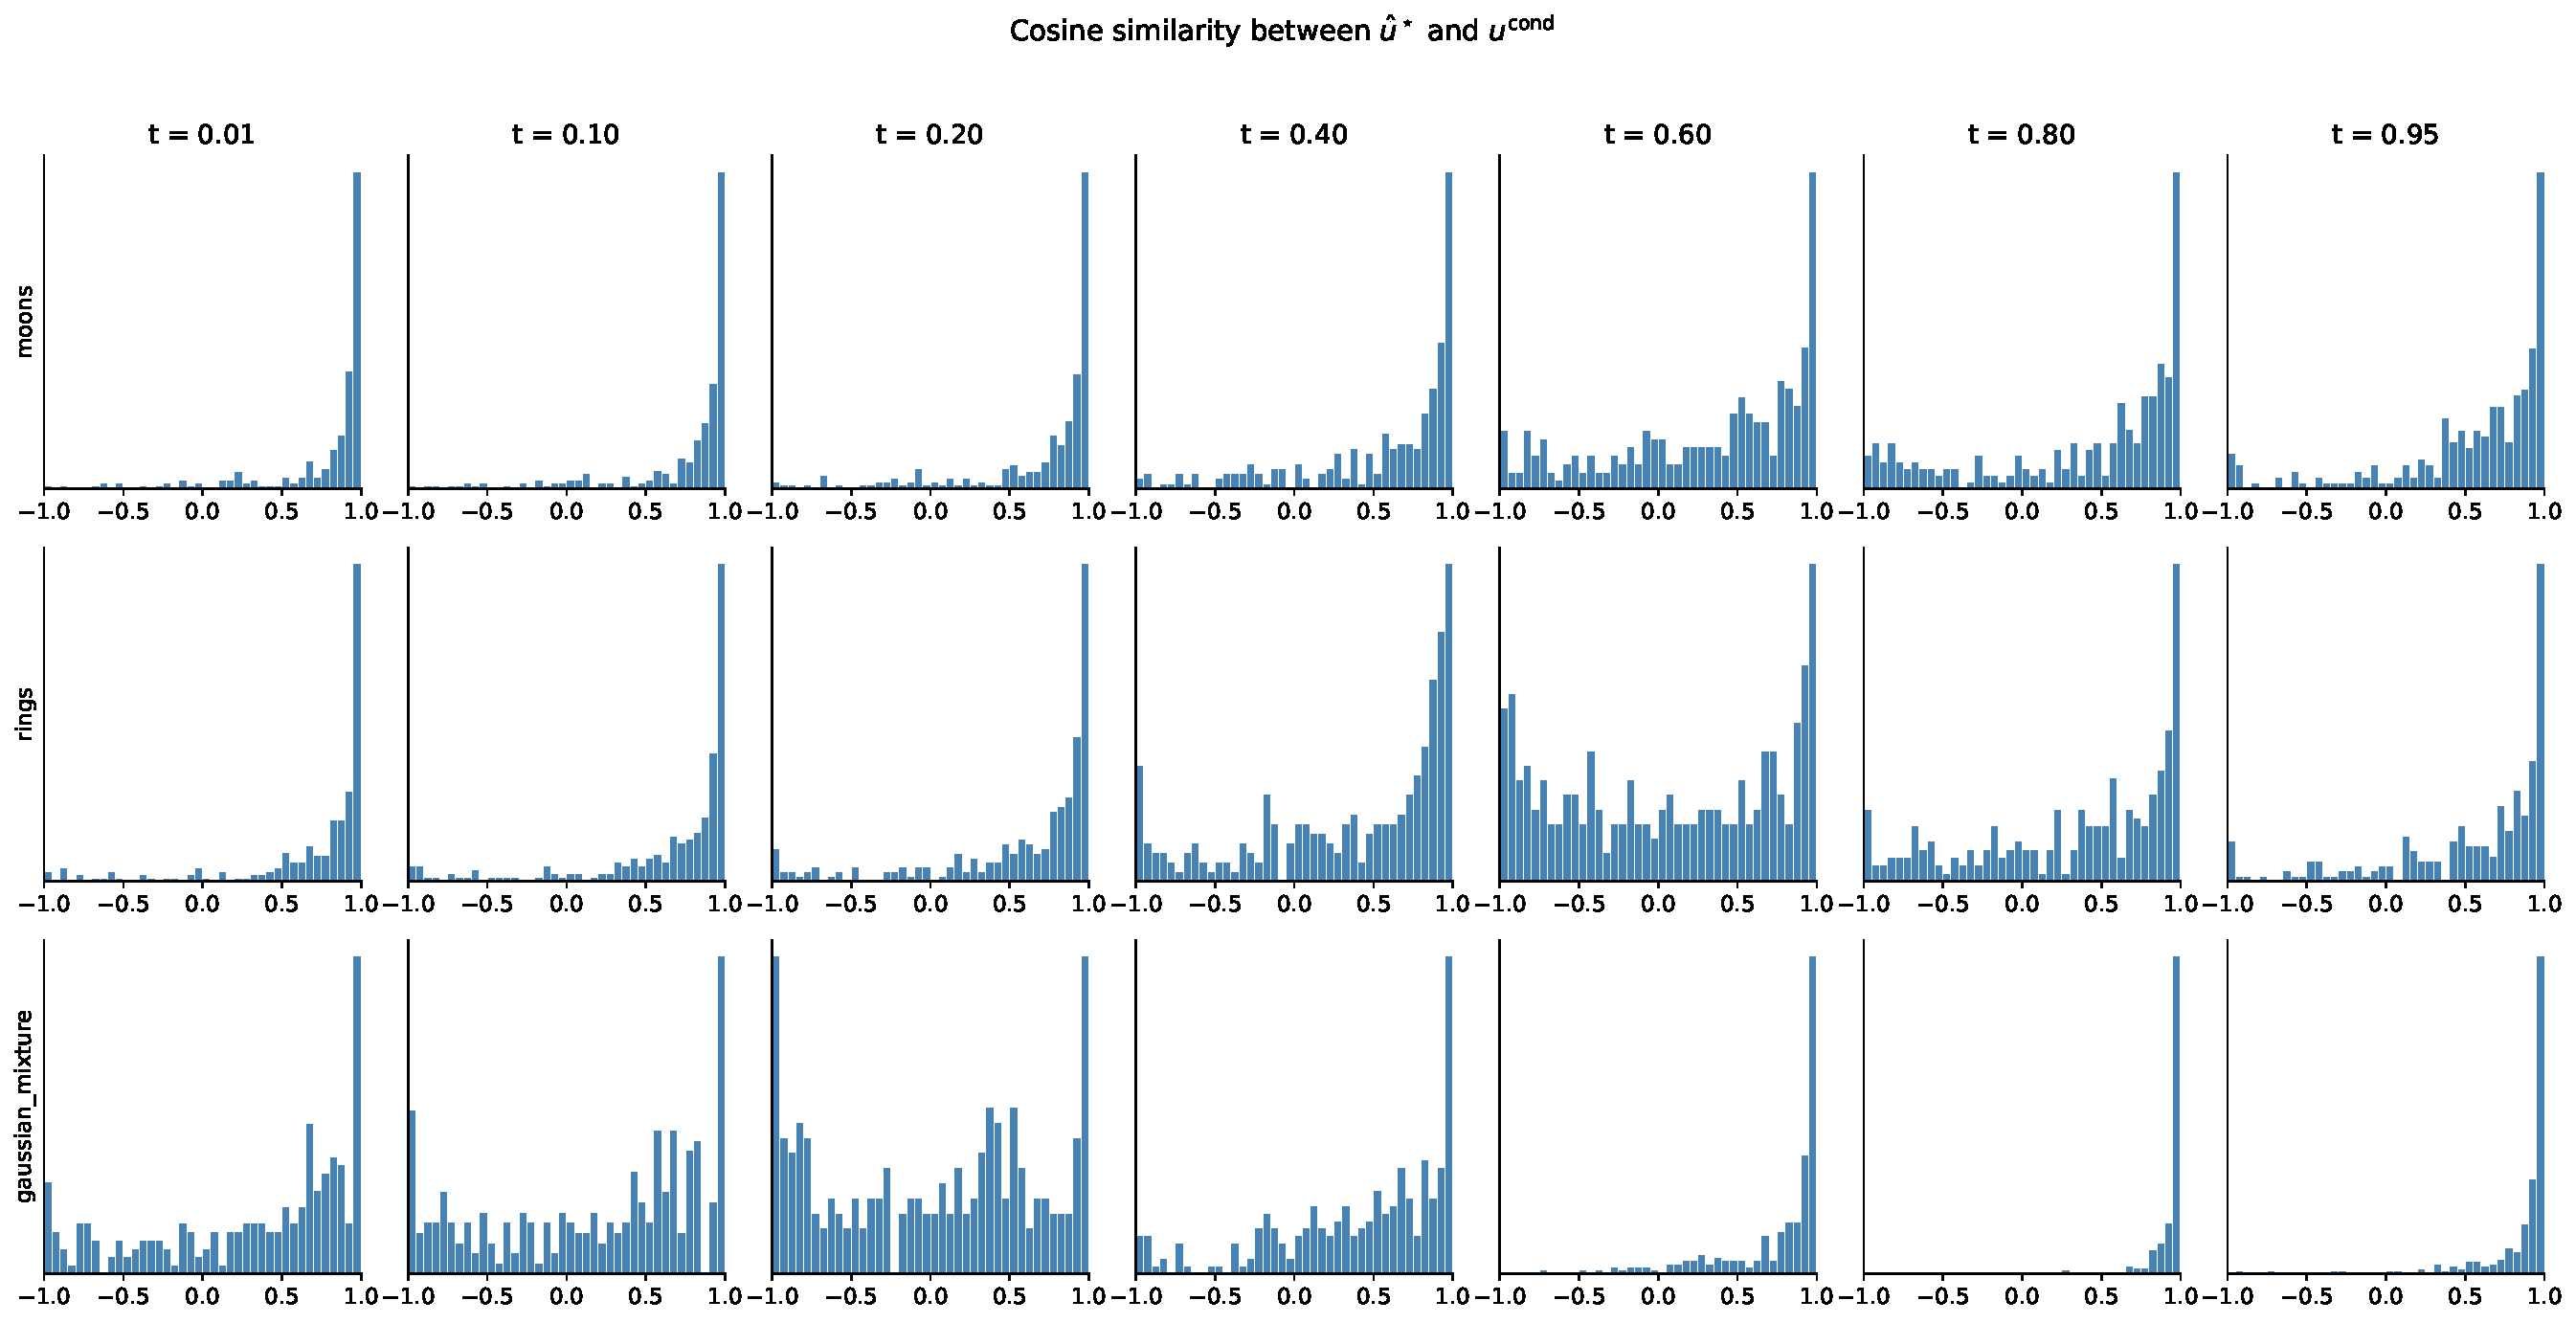
\includegraphics[width=0.82\textwidth]{figs/notebook_1/fig1a_cosine_histograms-2.pdf}
\caption{Cosine similarity histograms between $\hat{u}^\star$ and $u^{\mathrm{cond}}$ for three 2D datasets ($n = 5000$) at various time steps.
The progressive concentration near~1 confirms the collapse to a single conditional direction.
In 2D the stochastic regime persists until intermediate~$t$, consistent with the paper's Figure~1a (top row, two-moons).}
\label{fig:cosine-hist}
\end{figure}

\begin{figure}[ht]
\centering
\begin{subfigure}[t]{0.46\textwidth}
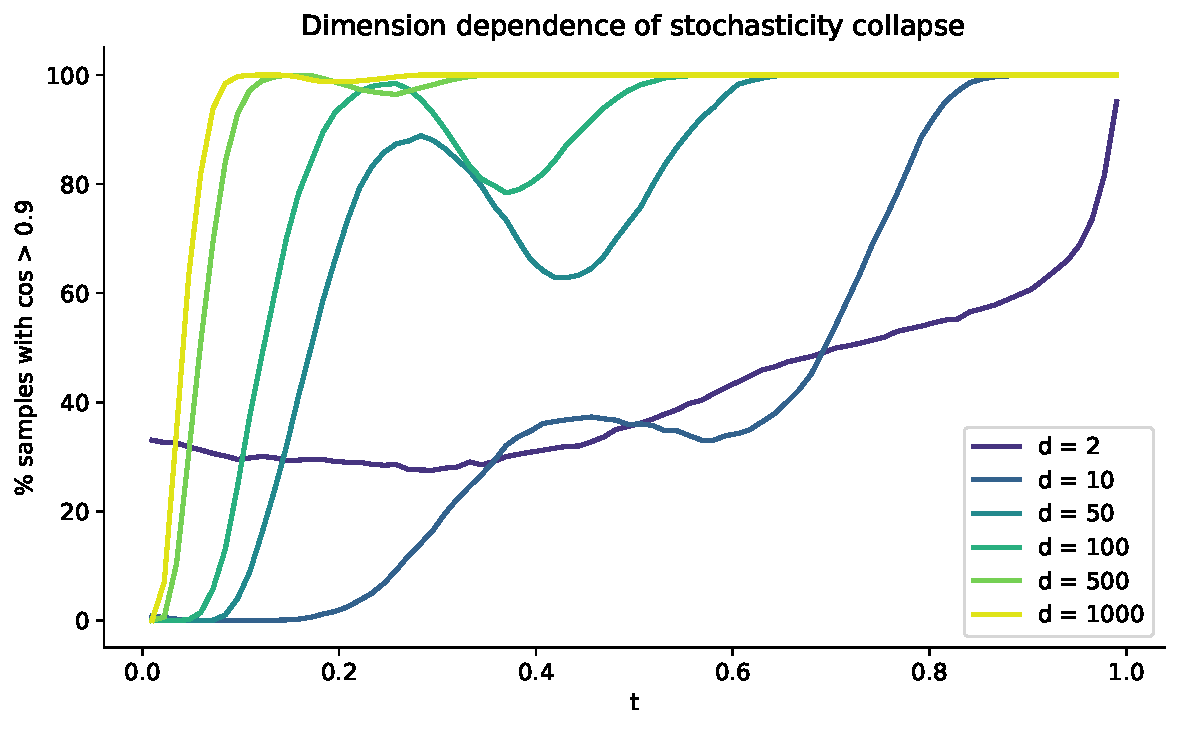
\includegraphics[width=\textwidth]{figs/notebook_1/fig1c_dimension_dependence-2.pdf}
\caption{Dimension dependence of the stochasticity collapse.}
\end{subfigure}
\hfill
\begin{subfigure}[t]{0.46\textwidth}
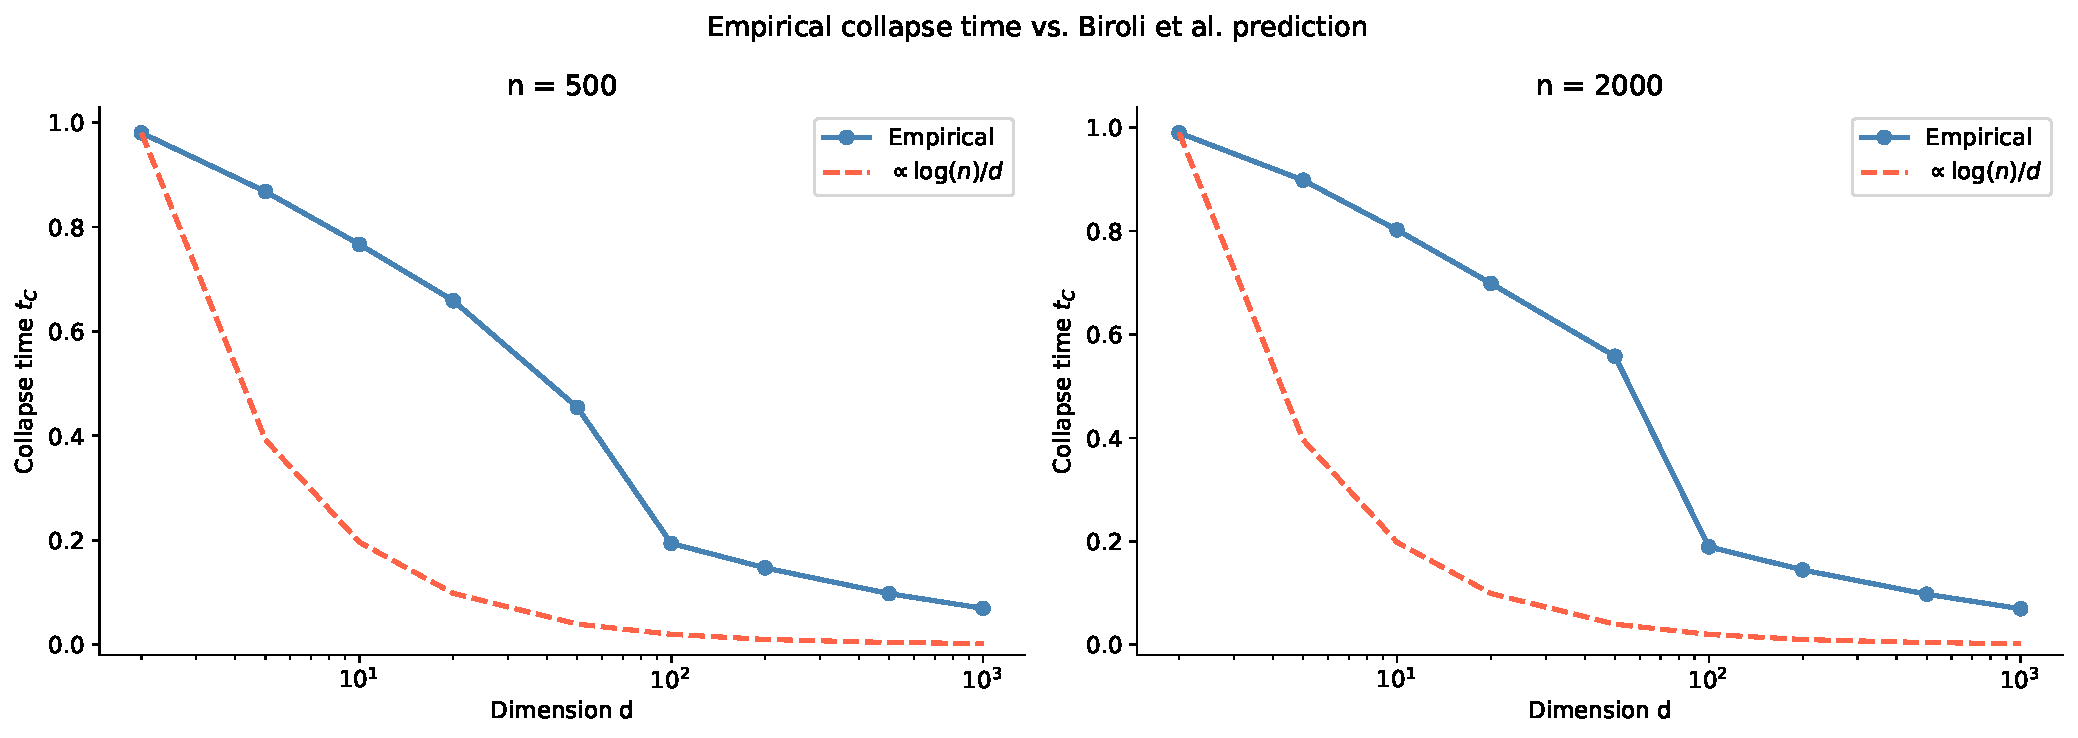
\includegraphics[width=\textwidth]{figs/notebook_1/fig1_collapse_time_vs_theory-2.pdf}
\caption{Empirical collapse time vs.\ Biroli et al.\ prediction.}
\end{subfigure}
\caption{(a)~Percentage of pairs with $\cos(\hat{u}^\star, u^{\mathrm{cond}}) > 0.9$ vs.\ $t$, for varying data dimension~$d$ ($n = 2000$).
Higher dimension leads to earlier collapse, consistent with the paper's Figure~1c on Imagenette.
(b)~Empirical collapse time matches the $\propto\!\log(n)/d$ scaling from~\cite{biroli2024dynamical} for both $n = 500$ and $n = 2000$.}
\label{fig:dim-dependence}
\end{figure}

\begin{figure}[ht]
\centering
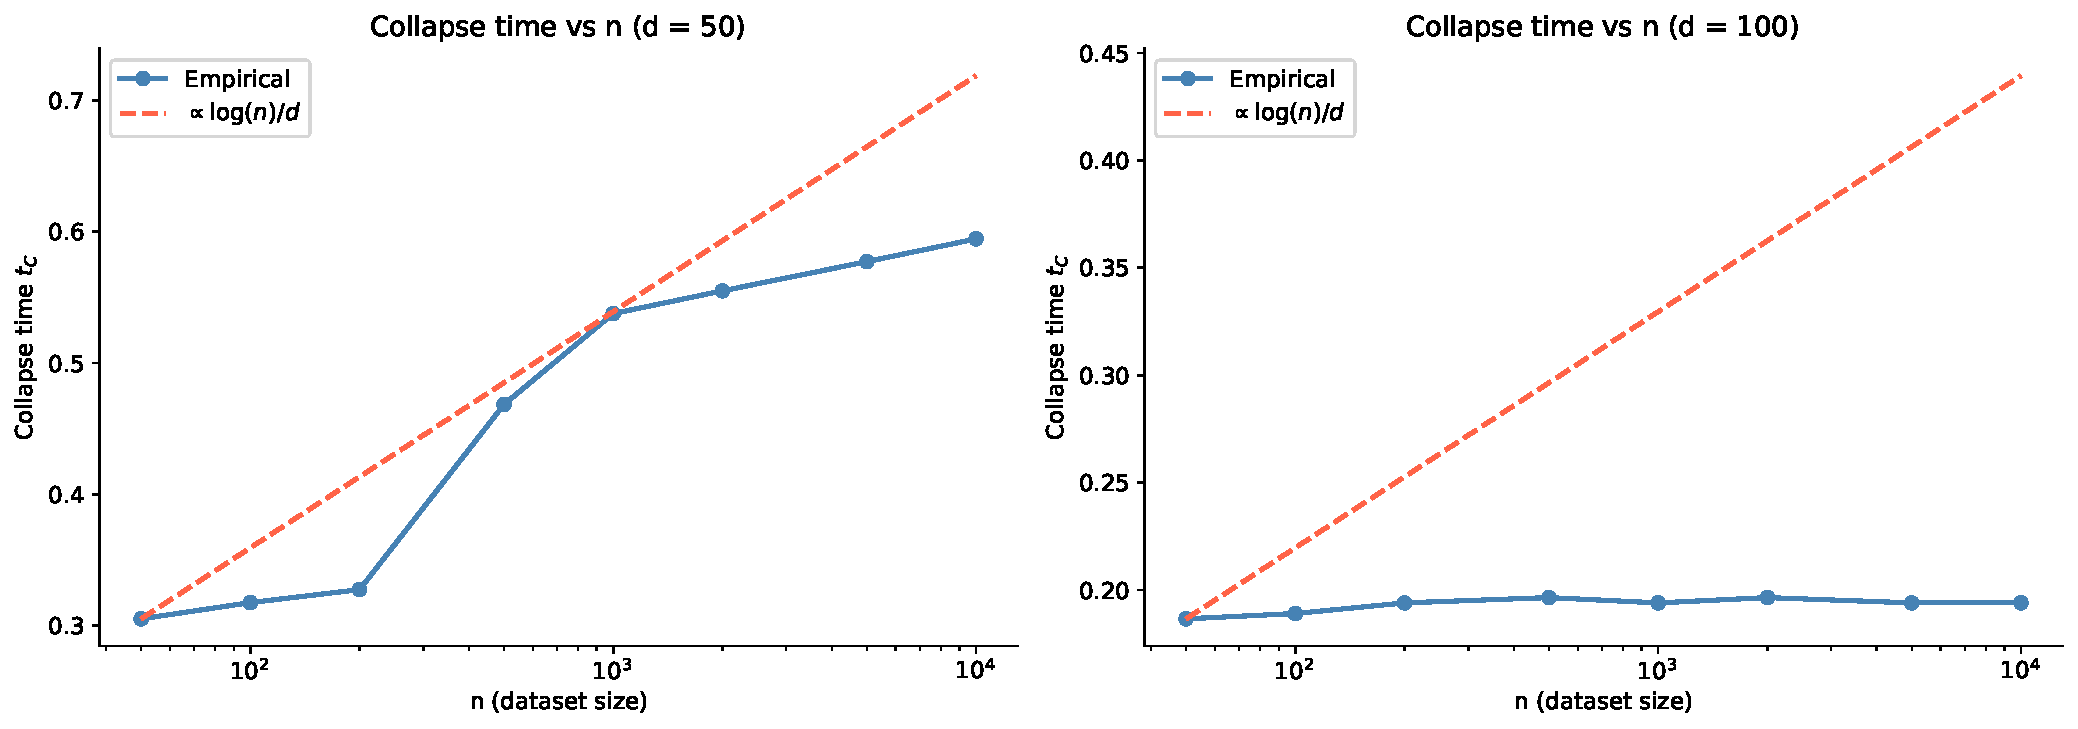
\includegraphics[width=0.55\textwidth]{figs/notebook_1/fig1_collapse_vs_n-2.pdf}
\caption{Collapse time $t_C$ vs.\ dataset size~$n$ at fixed $d = 50$ and $d = 100$.
The empirical values follow the $\propto\!\log(n)/d$ scaling (dashed line), confirming the logarithmic dependence on~$n$.}
\label{fig:collapse-vs-n}
\end{figure}

% ---- Figure 2 figures ----

\begin{figure}[ht]
\centering
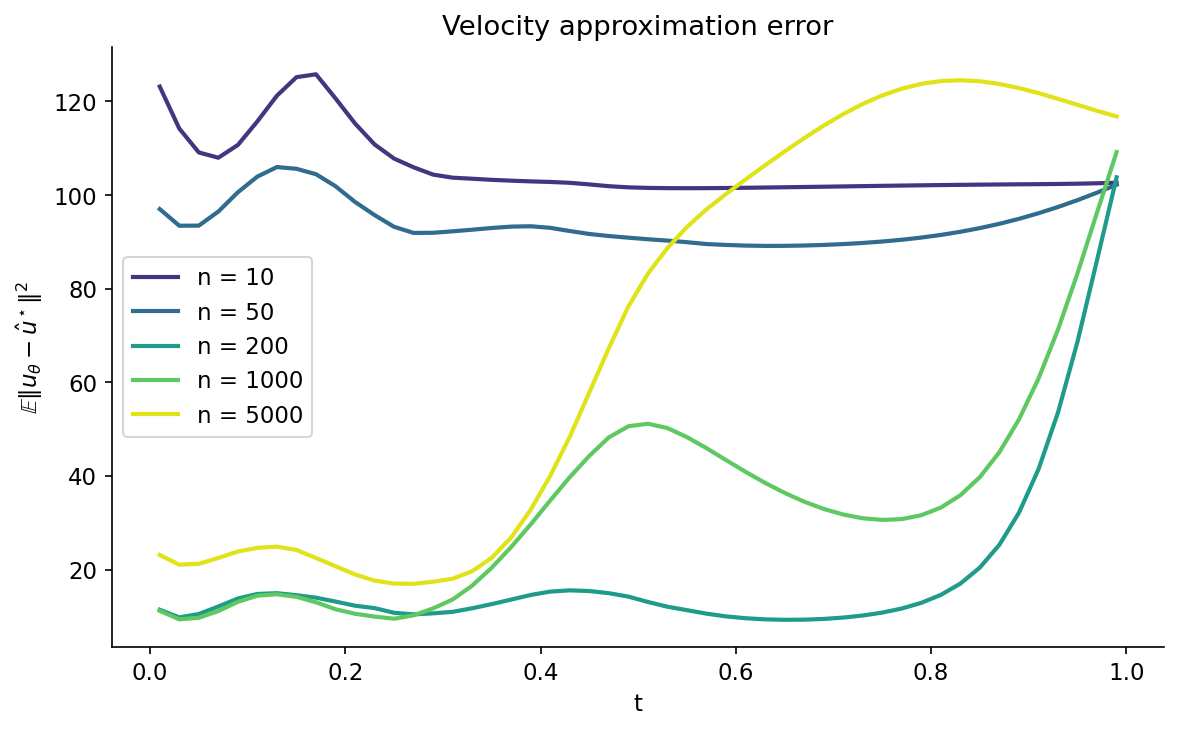
\includegraphics[width=0.62\textwidth]{figs/notebook_2/fig2.png}
\caption{Velocity approximation error $\E\norm{u_\theta - \hat{u}^\star}^2$ vs.\ $t$ for varying dataset sizes on the $d = 100$ Gaussian mixture.
Two failure zones are visible: an early-time bump at $t \approx 0.12$--$0.15$ (most prominent for $n = 10$), and a late-time rise for $n \geq 200$.}
\label{fig:velocity-error}
\end{figure}

\begin{figure}[ht]
\centering
\begin{subfigure}[t]{0.33\textwidth}
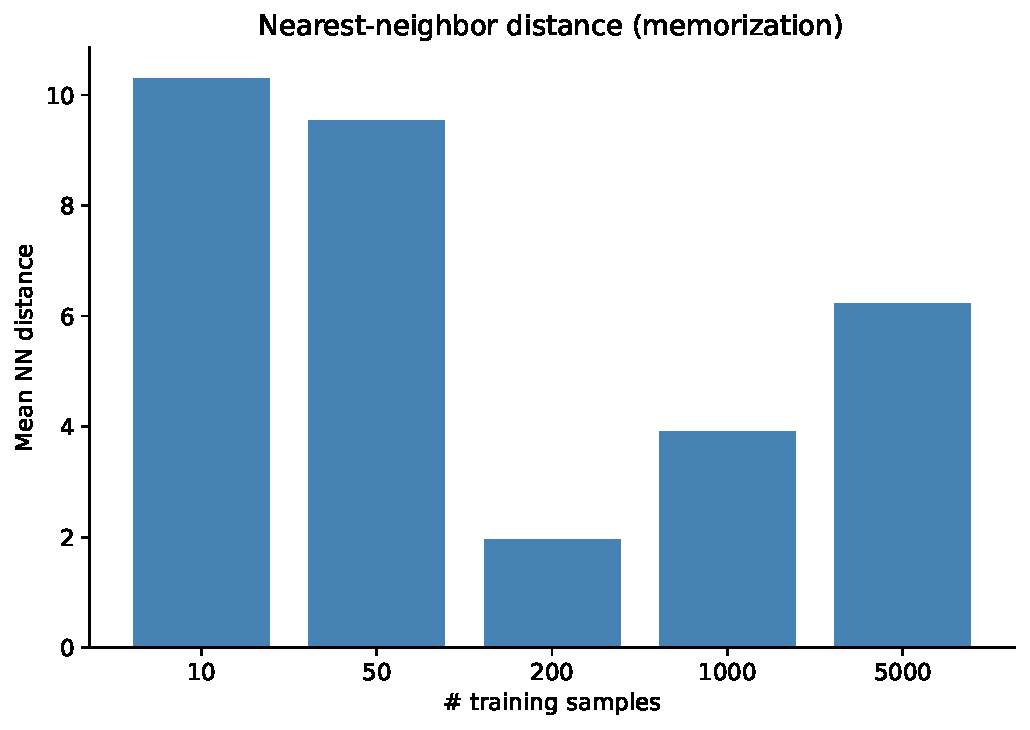
\includegraphics[width=\textwidth]{figs/notebook_2/fig2_right_nn_distance.pdf}
\caption{Mean nearest-neighbor distance.}
\end{subfigure}
\hfill
\begin{subfigure}[t]{0.57\textwidth}
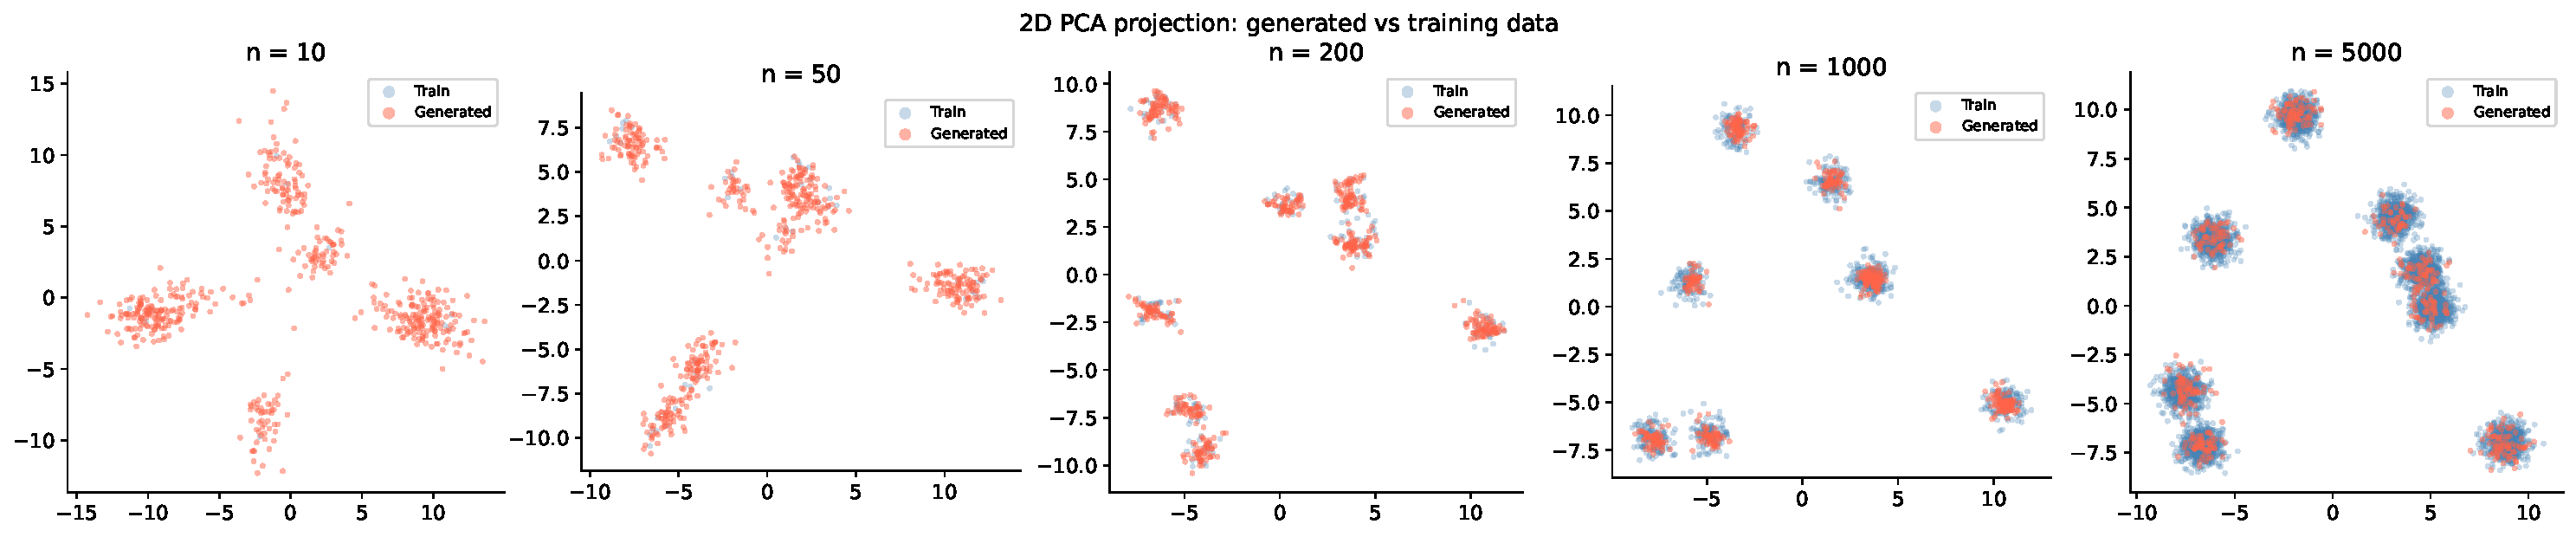
\includegraphics[width=\textwidth]{figs/notebook_2/fig2_scatter_comparison.pdf}
\caption{2D PCA projection of generated vs.\ training data.}
\end{subfigure}
\caption{(a)~The nearest-neighbor distance between generated and training samples increases with $n$, indicating a transition from memorization to generalization as the dataset outgrows the network's capacity.
(b)~PCA projections confirm the trend: for small $n$, generated points (red) cluster near training data (blue); for large~$n$, the model produces diverse samples with the same modal structure.}
\label{fig:nn-dist-scatter}
\end{figure}

% ---- Figure 3 figures ----

\begin{figure}[ht]
\centering
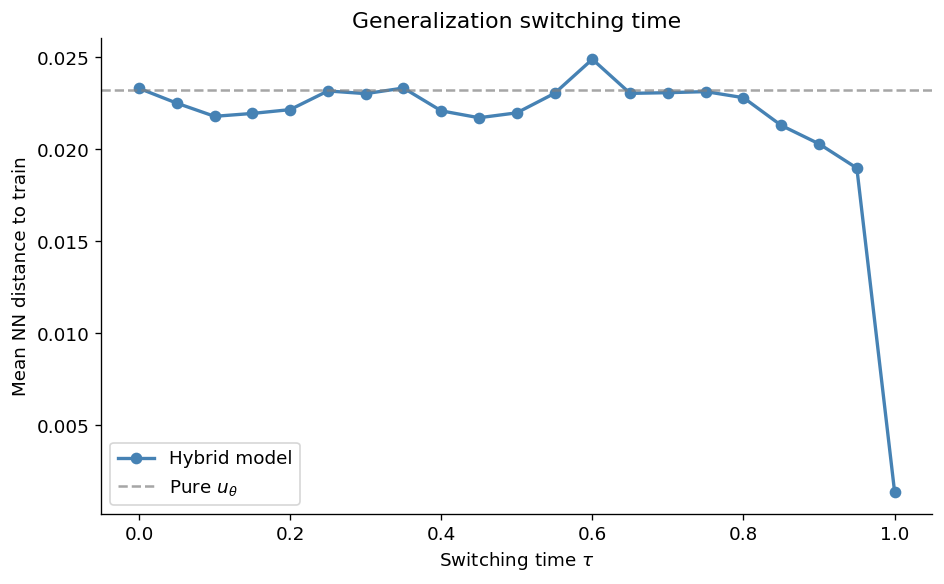
\includegraphics[width=0.44\textwidth]{figs/notebook_3/fig3_hybrid_switching.png}
\caption{Mean nearest-neighbor distance as a function of the hybrid switching time $\tau$ (2D Gaussian mixture, $n=2000$). Plateau for $\tau \leq 0.2$, sharp drop above $\tau \approx 0.35$.}
\label{fig:fig3-switching}
\end{figure}

\begin{figure}[ht]
\centering
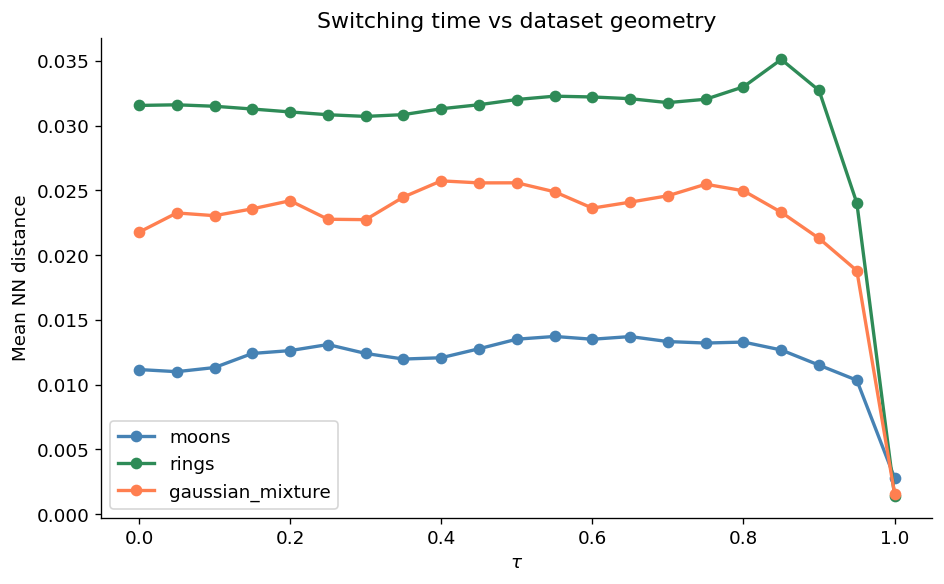
\includegraphics[width=0.50\textwidth]{figs/notebook_3/fig3_geometry_comparison.png}
\caption{Switching curves for three 2D geometries ($n=2000$). The switching time varies with dataset structure, reflecting the complexity of $\hat{u}^\star$.}
\label{fig:fig3-geometry}
\end{figure}

\begin{figure}[ht]
\centering
\begin{subfigure}[t]{0.46\textwidth}
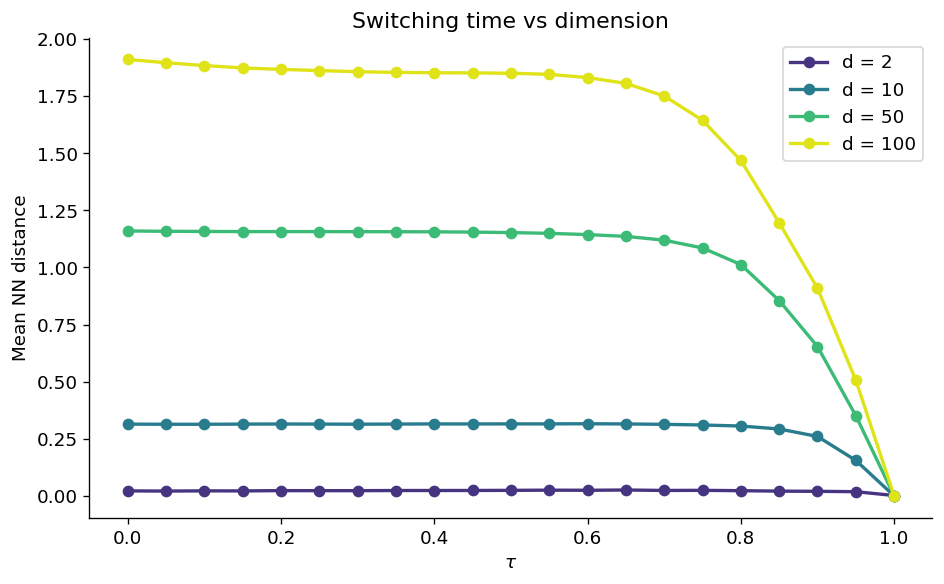
\includegraphics[width=\textwidth]{figs/notebook_3/fig3_dimension_scaling_low.png}
\caption{$d \in \{2, 10, 50, 100\}$.}
\end{subfigure}
\hfill
\begin{subfigure}[t]{0.46\textwidth}
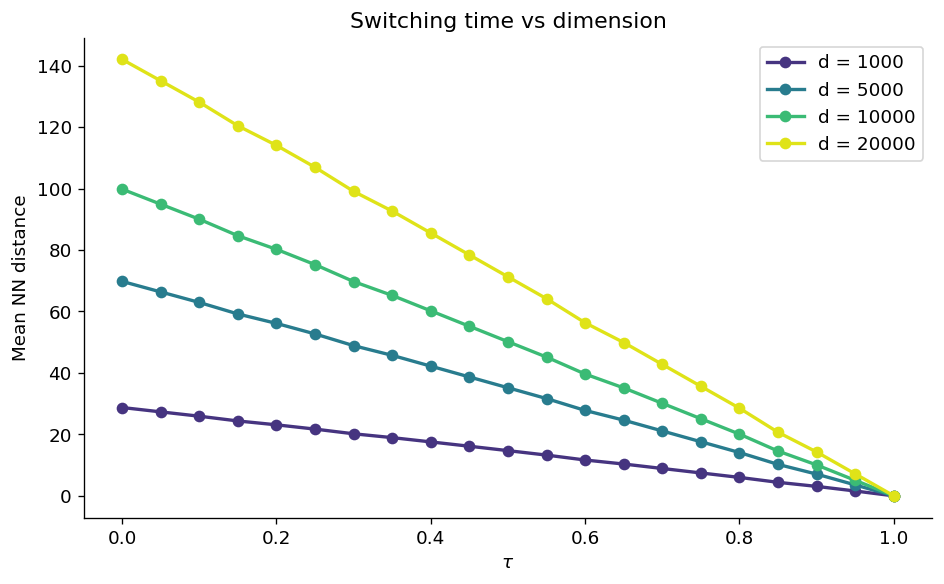
\includegraphics[width=\textwidth]{figs/notebook_3/fig3_dimension_scaling_high.png}
\caption{$d \in \{1000, 5000, 10000, 20000\}$.}
\end{subfigure}
\caption{Switching time vs.\ dimension. Left: switching point shifts earlier as $d$ grows. Right: at very high $d$, the curve is flat --- even $\hat{u}^\star$ generalizes, consistent with the $\mathcal{O}(\log n / d)$ collapse time scaling.}
\label{fig:fig3-dim}
\end{figure}

\begin{figure}[ht]
\centering
\begin{subfigure}[t]{0.46\textwidth}
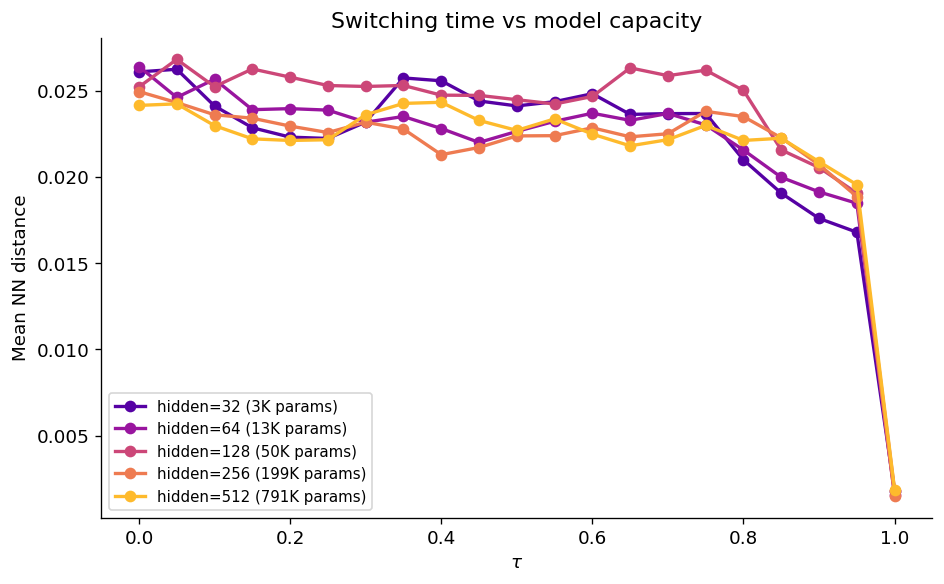
\includegraphics[width=\textwidth]{figs/notebook_3/fig3_capacity.png}
\caption{Effect of model capacity (hidden dim).}
\label{fig:fig3-capacity}
\end{subfigure}
\hfill
\begin{subfigure}[t]{0.46\textwidth}
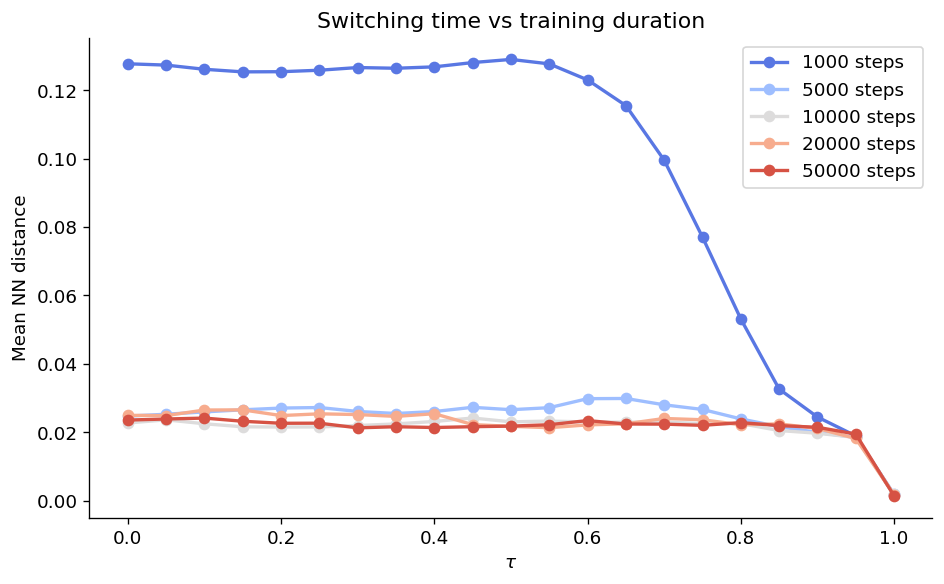
\includegraphics[width=\textwidth]{figs/notebook_3/fig3_training_duration.png}
\caption{Effect of training duration (\# steps).}
\label{fig:fig3-training}
\end{subfigure}
\caption{Switching curves varying model capacity (left) and training duration (right) on the 2D Gaussian mixture. Larger/longer-trained models memorize better, confirming that generalization is a consequence of limited expressiveness.}
\label{fig:fig3-ablations}
\end{figure}

% ---- Notebook 4 figures ----

\begin{figure}[ht]
\centering
\begin{subfigure}[t]{0.46\textwidth}
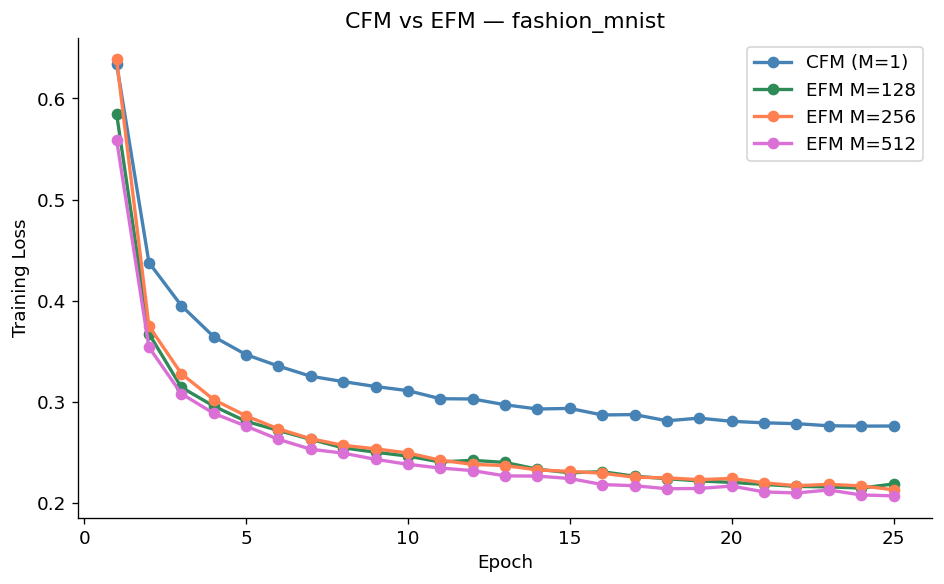
\includegraphics[width=\textwidth]{figs/notebook_4/fig4_training_loss.png}
\caption{Training loss (CFM vs EFM, $M\in\{128,256,512\}$).}
\label{fig:fig4-loss}
\end{subfigure}
\hfill
\begin{subfigure}[t]{0.46\textwidth}
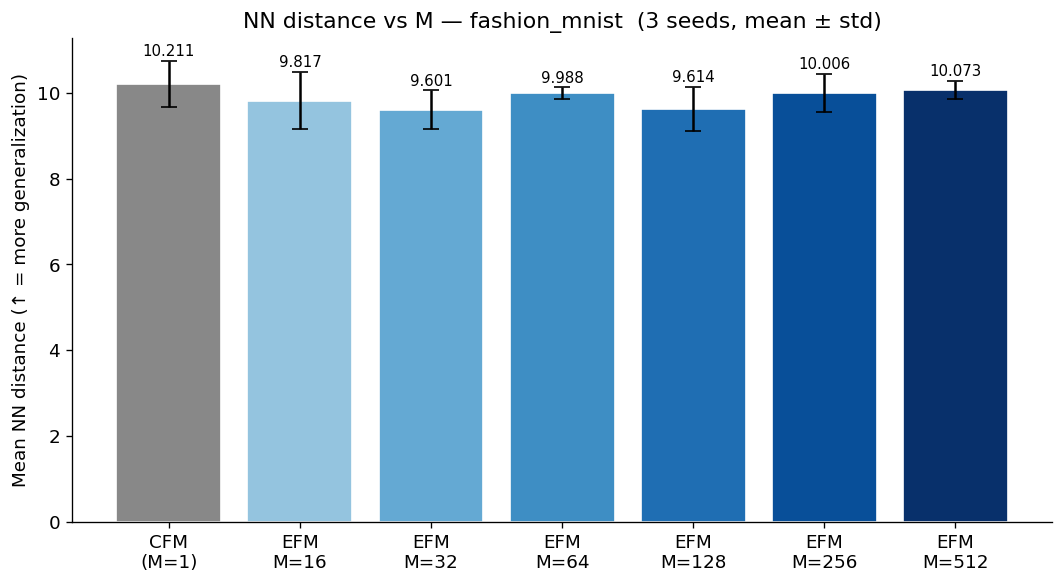
\includegraphics[width=\textwidth]{figs/notebook_4/fig4bis_M_sweep.png}
\caption{NN distance $\pm$ std (3 seeds) vs.\ $M$.}
\label{fig:fig4bis-sweep}
\end{subfigure}
\caption{Fashion-MNIST experiments. EFM achieves lower training loss but identical NN distances across all~$M$, confirming that target stochasticity does not drive generalization.}
\label{fig:fig4-combined}
\end{figure}

\end{document}
